\chapter{System-Architektur}\label{chap:architecture}

In diesem Kapitel wird die praktische Umsetzung des in \vref{chap:concept} beschriebenen Konzeptes von Specios betrachtet; die Implementierung eines Supera Specios\index{Supera Specios}.

\section{Verwaltung}\label{sec:maintenance}

Das Grundprinzip ist mit der Wikipedia vergleichbar: Das System ist interaktiv und multilingual, die Daten werden von den Mitgliedern über eine Internetzugang erstellt (siehe dazu auch \textit{Schwarmauslagerung} und \textit{Schwarmintelligenz}).

\subsection{Lokalisierung}\label{sec:maintenance/localization}

Da das Systeme für alle Menschen mit den selben Inhalten zugänglich sein muss, habe ich für einfache Ausdrücke (Bezeichnungen, kurze Erklärungen udgl.) ein dynamisches Sprachsystem entwickelt, welches folgende Merkmale aufweist:
\begin{itemize}
\item Ausdrücke können initial in einer beliebigen Sprache formuliert werden.
\item Mitglieder können Ausdrücke jederzeit in ihre eigene oder eine andere Sprache übersetzen.
\item Mitglieder können eine priorisierte Liste ihrer beherrschten Sprachen erstellen, sodass jeweils automatisch die am besten passendste Übersetzung ausgewählt wird. Die Übersetzungsvorschrift wird standardmäßig von den im Internetbrowser eingestellten Sprachen abgeleitet. Im Folgenden sehen Sie eine beispielhafte Übersetzungsvorschrift für die Spracheinstellung \verb|de,en,es-cl|:
  \begin{compactenum}[1.]
  \item \textit{de"=DE: deutsch (Deutschland)}.
  \item Der älteste Ausdruck aller anderen deutschen Dialekte wie \textit{de"=AT: deutsch (Österreich)}.
  \item \textit{en"=US: English (United States)}.
  \item Der älteste Ausdruck aller anderen englischen Dialekte wie \textit{en"=GB: Englisch (United Kingdom)}.
  \item \textit{es"=CL: español (Chile)} -- weil in der Spracheinstellung direkt angegeben.
  \item \textit{es"=ES: español (España)}.
  \item Der älteste Ausdruck aller anderen spanischen Dialekte.
  \item Der älteste Ausdruck aller anderen Sprachen.
  \end{compactenum}
\item Über Übersetzungsvorschläge kann direkt an Ort und Stelle in einem kontextsensitiven Bearbeitungs"=Menü abgestimmt werden.
\item Intelligente Zielsprachauswahllisten bei der Erstellung von Übersetzungen (basierend auf bereits vorhandenen Übersetzungen und persönlichen Sprachpräferenzen).
\end{itemize}

Das Sprachsystem verwendet derzeit MySQL, was für eine riesige Datenmenge an Ausdrücken vermutlich ungeeignet ist. Zumindest die Abstimmungen müssen in ein leistungsstärkeres Datenbanksystem ausgelagert werden, wobei dann auf das derzeit vorhandene direkte Feedback bei Änderungen wahrscheinlich verzichtet werden muss. Siehe dazu \vref{sec:database}.

\subsection{Wahlsystem}\label{sec:maintenance/voting}

\begin{figure}
\caption[Wahlsystem (Übersicht)]{Gelb: Über Regeln und Aktionsvorschläge wird kompetenzgewichtet abgestimmt. Grün: Aktuelle Ressourcen, Gesetzmäßigkeiten und Tatsachen werden demokratisch katalogisiert.}
\label{fig:choices}
\begin{center}
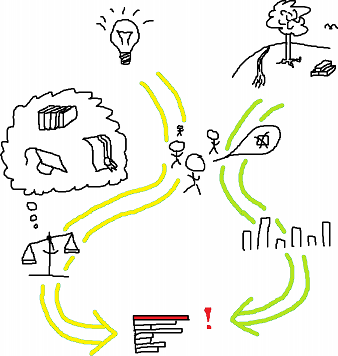
\includegraphics[width=0.75\textwidth]{../gfx/speciosgraph2_small.png}
\end{center}
\end{figure}

Mit Hilfe des Wahlsystemes entscheidet jedes Mitglied über grundlegende Dinge und Daten bzw. definiert sie, siehe \vref{fig:choices}. Daraus baut das System mit Hilfe von ebenfalls gewählten einfachen Formeln oder komplexen Skripten diverse Zusammenhänge zwischen den Daten auf, welche mit Hilfe einer künstlichen Intelligenz (siehe \vref{sec:ki}) möglichst effektiv zu Regeln und Handlungsempfehlungen synthetisiert werden.

Es können verschiedene Daten zum selben Sachverhalt eingetragen werden, wobei jedes Datum an mindestens ein Mitglied gebunden ist. Dadurch wird eine dynamische Abstimmung zu jedem Sachverhalt ermöglicht.

Zum Schutz vor Fehlinformationen aufgrund von Unwissenheit oder Meinungen aus dem Bauchgefühl heraus, gibt es zwei Lösungen: Zum einen werden vom System abstrahierte Sachverhalte, welche auf spezielleren, grundlegenderen Daten beruhen, höher bewertet als allgemeine Aussagen. Zum anderen werden die Qualifikationen des Wählers berücksichtigt, welche zur Erfassung des jeweiligen Sachverhaltes benötigt werden (Kompetenzwichtung). Diese werden von anderen Mitgliedern (z.B. Lehrern, Professoren udgl.) geliefert und müssen verifiziert werden, bzw. ergeben sich aus Zeugnissen oder sonstigen Leistungsnachweisen.

\subsubsection{Benutzerschnittstelle}

In einer persönlichen Übersicht wird jeder Mensch einsehen können, welche seiner Eingaben nicht mit den aktuellen Festlegungen übereinstimmen, um sie ggf. zu korrigieren oder die entsprechende Stimme zu entfernen. Umgekehrt werden "`unsichere"' Daten, die zwar auf mehrheitlichen oder fundamentaleren Ansichten basieren, aber (soweit möglich automatisch korrigierte) Konflikte mit anderen Daten aufweisen oder eine nicht zu vernachlässigende Menge an Gegenmeinungen besitzen, hervorgehoben, damit strukturelle Fehler, neue Erkenntnisse oder alternative Betrachtungen Aufmerksamkeit erhalten.

\subsubsection{Durchmischtes}

ich glaub ich mach das so:

1) daten oder datenblöcke (intern dasselbe, aber der verbund muss wiedererkennbar sein, um blockweise wahlen zu ermöglichen) über alles mögliche, aber immer mit orts-, zeitraum- und genauigkeits-angaben können von jedem benutzer über spezielle webinterfaces oder über eine API eingetragen werden. jeder benutzer kann daten über dieselbe sache in derselben orts- und zeit-ebene nur 1x im system haben, darf sich auch nicht überschneiden. wenn ein benutzer die daten einer anderen person wählt, ist das logisch (und vielleicht auch technisch) dasselbe als würde er eben diese daten von sich aus einfügen.

2) auf magische weise werden dann mehrheits- und kompetenzgewichtungen reingeworfen, überschneidungen und konflikte aufgelöst (besonders lustig bei zahlendaten) und am ende stehen dann die besten vorschläge da.

3) in einem schritt, vielleicht demselben, werden dann konflikte zwischen abstraktionsschichten irgendwie aufgelöst, diese überhaupt zu finden ist vielleicht auch nicht gerade einfach. und untere schichten müssen auf alle oberen vereinfacht werden.

4) ein problem ist bei dem ganzen kram, dass bestimmte operationen vorzugsweise unmittelbar vom system bearbeitet werden müssen, z.b. übersetzungen von wörtern müssen sofort übernommen werden, das einfügen neuer daten sollte sofort sichtbar sein, usw.

5) und dann kommt die richtige magie, lauter demokratisch ermittelte scripte, die zusammenhänge zwischen den rohdaten herstellen und höhere tatsachen definieren. z.b. die wichtigkeit der spezies mücke bezogen auf dessen intelligenz und der anzahl lebender exemplare in deutschland oder so. diese scripte generieren also neue daten, die die "richtigkeit" der baiserenden daten mit einbeziehen muss, damit falls sie neue daten definieren für die es bereits manuelle meinungen gibt, wieder neu entschieden werden kann was denn nun korrekt ist - klingt kompliziert.

6) und zum schluss muss specios aktions-skripte und dessen auswirkungen über die zeit simulieren, um zu ermitteln wie am ende die basisziele maximal erfüllt werden. für einen gedanken muss ggf. alles ab punkt 3 wiederholt werden. ungenaue aber schneller ableitbare folgen mit entsprechend schlechteren wahrscheinlichkeiten erhöhen dabei die arbeitsgeschwindigkeit, also muss der kompromisse zwischen zeit, genauigkeit und wichtigkeit fällen.
klingt das machbar?

\subsection{Sicherheit}\label{sec:maintenance/security}

Vor Manipulationen kann man sich mit Hilfe verteilter Gegenrechnungen, zertifizierter Snapshots und spezieller Notpläne schützen, welche zeitlich begrenzte Gültigkeit besitzen. Mit Notplänen sind (gedruckte) zertifizierte Repräsentationen der wesentlichen abstrahierten Regeln gemeint, welche in jedem Haushalt oder ähnlichen, möglicherweise größeren Gruppierungen gehalten und durch einen sicheren, möglichst persönlichen Mehrheitsentscheid aktiviert werden können.

\section{Künstliche Intelligenz}\label{sec:ki}

Die künstliche Intelligenz (KI) muss die Folgen möglicher Tätigkeiten simulieren und daraus notwendige Handlungen berechnen. Da dies ziemlich rechenaufwendig ist, besteht das Hauptproblem darin, einen Kompromiss zwischen Prioritäten, Zeit und Abstraktionsebene zu finden und Berechnungen je nach Notwendigkeit nach und nach verfeinern und optimieren zu können. Die vorrausschauende Planung der notwendigen Berechnungen ist dabei von zentraler Bedeutung.

Die Arbeitsweise kann in folgende Prozesse eingeteilt werden:
\medskip
\begin{compactitem}
\item Wahlprozess (siehe \vref{sec:maintenance/voting})
\item Konfliktkorrekturprozess
\item Zusammenführungsprozess
\item Auswertungsprozess
\item Abstrahierungsprozess
\item u.\,a.
\item Simulationsprozess
\end{compactitem}
\medskip

Die verschiedenen Prozesse werden im Folgenden näher beschrieben.

\subsection{Simulationsprozess}\label{sec:ki/simulation}

Die KI führt Effizienz"=Abschätzungen durch, wobei für mögliche Tätigkeiten und Betrachtungen jeweils die Wahrscheinlichkeit berechnet wird, wie zielführend eine nähere Untersuchung sein wird. Im Endeffekt wird fortwährend versucht die erwartete Wahrscheinlichkeit, Grundgesetze einzuhalten, und variable Systemparameter (wie der Wohlstand von Systemmitgliedern und anderen Lebewesen, siehe dazu \vref{sec:basis/aim}) auf lange Sicht zu maximieren.

Dazu werden mögliche Aktionskombinationen nicht willkürlich durchprobiert, sondern sie werden anhand der Zieldefinitionen und diverser Wahrscheinlichkeitsfaktoren errechnet und dynamisch verfeinert, so dass das System jederzeit mit der maximal denkbaren Fortschrittsgeschwindigkeit läuft. Um wegen chaotischem Verhalten von Aktionen oder Fehlern nicht fehlgeleitet zu werden, werden suboptimale Lösungswege sowie zufällig gewählte parallel analysiert, je nach Priorität der Kernanalyseaufgaben.

\subsubsection{Daten}

Viele Daten besitzen zusätzlich Orts"~, Zeit"~/""Gültigkeits"~ und Genauigkeits"=Angaben.

\subsubsection{Durchmischtes}

ich glaube die implementierung von specios würde einer ki wie ich/falk sie bisher halbwegs geplant haben ziemlich nahe kommen müssen:
z.b. muss es informationen verallgemeinern können (aus effizienzgründen), abschätzen welchen fehler informationen haben und ggf. spezialisieren/neu berechnen. dafür muss es aber hoffentlich nicht unbedingt informationen in zusammenhang setzen oder neue informationen ableiten, das ist ja mehr oder weniger der demokratische akt: meinungen sammeln, zusammenhänge aufbauen, gesetze formulieren. das system zeigt quasi nur auf abstrakter weise auf was sache ist und was getan werden muss.
und es muss aktivitäten simulieren, was auswirkungen auf sämtliche daten hat und erkenntnisse zulässt.
das hauptproblem neben der spezifikation ist vermutlich der denkvorgang mit dem beschränkten arbeitsspeicher.

\section{Datenbanksystem}\label{sec:database}

Es ist ein dokumentbasiertes Datenbanksystem erforderlich, bei dem jeder Datenpunkt durch eine Datei repräsentiert wird. Aufgrund der Menge an Daten ist ein kompliziertes Verwaltungssystem erforderlich, welches einfach überschaubar und handhabbar ist. Sämtliche Hilfssysteme wie ein Indizierungssystem müssen optional sein. D.\,h. das Datenbanksystem muss sich bei Problemen vollständig selbst rekonstruieren können, sofern die jeweilige Datendateien oder Sicherungen von Ihnen zugänglich sind.
